\documentclass[a4paper,12pt]{article}

\usepackage{geometry}       % Required for page layout.
\usepackage{hyperref}       % Required for hyperlinks.
\usepackage{graphicx}       % Required for figures.
\usepackage{subfig}         % Required for minipages.


\usepackage{amsmath}
\usepackage{amsfonts}
\usepackage{amssymb}
\usepackage{amsthm}
\usepackage{float}

\usepackage{hyperref}
\usepackage{listings}
\usepackage{xcolor}

\definecolor{codegreen}{rgb}{0,0.6,0}
\definecolor{codegray}{rgb}{0.5,0.5,0.5}
\definecolor{codepurple}{rgb}{0.58,0,0.82}
\definecolor{backcolour}{rgb}{0.95,0.95,0.92}

\lstdefinestyle{mystyle}{
    backgroundcolor=\color{backcolour},   
    commentstyle=\color{codegreen},
    keywordstyle=\color{magenta},
    numberstyle=\tiny\color{codegray},
    stringstyle=\color{codepurple},
    basicstyle=\ttfamily\footnotesize,
    breakatwhitespace=false,         
    breaklines=true,                 
    captionpos=b,                    
    keepspaces=true,                 
    numbers=left,                    
    numbersep=5pt,                  
    showspaces=false,                
    showstringspaces=false,
    showtabs=false,                  
    tabsize=2
}

\lstset{style=mystyle}
\lstset{numbers =none}


\newgeometry{vmargin={25.4mm}, hmargin={27mm,27mm}}
\setlength\parindent{0pt}   % Disable paragraph indent.

\title{Cellular automaton traffic model of multi-lane highway}
\author{Axel Kierkegaard}
\usepackage{float}
\usepackage{makecell}
\begin{document}
\maketitle

\section{Introduction}
In a world dependent on transportation, traffic modeling is an essential tool to enable development of correctly dimensioned infrastructure. In this report the goal is to develop a model simulating a multi-lane highway and study the traffic flow for different number of lanes. Some of the questions we will investigate are:

\begin{itemize}
  \item \textbf{How does the road capacity compare for different number of lanes?}
  This is important when the knowledge of traffic flow along a specific route is to be used to design a road with a sufficient number of lanes to carry that traffic.
  \item \textbf{For a multi-lane highway - how does the fraction of cars and mean velocity in respective lanes depend on the density of cars?} Some say passing (left) lanes, supposed to be the fastest moving, are actually slower in heavy traffic.\footnote{Los Angeles Times, \textit{Experts Find No Easy Answers to Lane Phenomenon}, \url{https://www.latimes.com/archives/la-xpm-1992-04-13-me-189-story.html}}
  \item \textbf{How does the distribution of maximum velocities affect the flow rate?} The model will use cars with different maximum speeds. It is interesting to investigate how a more widely spread distribution of velocities affect the flow rate, and if the effect is the same for one lane as for several.
\end{itemize}

\section{Model description}
A cellular automaton model using discrete time steps will be used. The system is initialized with a fixed road length, number of lanes and cars, with periodic boundary conditions. This is a simplification since a normal highway has a start, entries and exits and an end, but implementing these would be difficult since the flow rate in these inlets/outlets determines the flow on the road. Using periodic boundary conditions instead keeps the model from getting too complicated. Another important part is the velocity distribution. To resemble real-life scenarios, the cars need different maximum speeds $v_{i, max}$. These are assumed to be normally distributed, which has been shown to be the case in some studies.\footnote{Roy, Saha, Sarkar, \textit{Speed Distributional Trends on Two-lane Roads with Mixed Traffic under Heavy Flow}, \url{https://www.sciencedirect.com/science/article/pii/S1877705817319318?ref=pdf_download&fr=RR-2&rr=787cc9874e7a991b}}\\

The rules that determine the behavior of the cars in every time step, looped over all cars $i=1,...,n_{cars}$ separately in this order are:

\begin{enumerate}
	\item If $v_i < v_{i, max}$ increase the velocity of car $i$, $v_i \rightarrow v_i+1$.
	\item Compute the distance $d_f$ from car $i$ to the closest car in front. 
	\begin{enumerate}
		\item If car $i$ travels the leftmost lane and $v_i \geq d_f$, reduce the velocity $v_i \rightarrow d_f-1$. 
		\item If car $i$ is not in the leftmost lane and $v_i \geq d_f$, calculate the distance to the closest car in front ($d_{fl}$) and behind it ($d_{bl}$) in the lane to the left. If $d_{fl}>d_f$ and $d_{bl}>v_{bl}$ car $i$ will switch to the left lane. Here $v_{bl}$ is the velocity of the car behind in the left lane. The velocity is then decreased if it is not smaller than the distance to the closest car in front, as in (a). 
		\item If car $i$ is not in the rightmost lane and $v_i < d_f$, calculate the distance to the closest car in front ($d_{fr}$) and behind it ($d_{br}$) in the lane to the right. If $d_{fr}>v_i$ and $d_{br} > v_{br}$ car $i$ will switch one lane to the right. Here $v_{br}$ is the velocity of the car behind in the right lane.
	\end{enumerate}
	
\item With probability p, decrease the velocity of car $i$, $v_i \rightarrow v_{i}-1$ if $v_i>0$. 
\item Update the position $x_i(t+1) = x_i(t) +v_i$
\end{enumerate}

The rules for lane changing are interesting, since this is a complex phenomenon in reality. It is reasonable that a driver switches lane to the left if there is more space there and the driver in front is driving too slow (rule 2b), and that they switch back to the right when there is enough space again (2c). However, a more advanced model should also encompass that (approximated) velocities and distances to cars further ahead are also taken into consideration when driving in real life. At the same time, a model fully implementing these factors would require more details of decision making, sight conditions on the road etc. making the model far too complicated.\\

Another important condition for lane changing to be allowed is that the velocity of the closest car behind in the new lane is smaller than the distance to said car. In real life, there are of course some drivers who switch lanes without "checking behind", but allowing that here would cause nonphysical scenarios. For example, a car with a very low velocity (or even 0) could change lane causing a car behind to brake from max speed to 0 in a single time step.\\

In the third step, the velocity of a car is reduced with a probability p. Too simulate a highway this probability should be rather low since cars generally try to uphold a constant velocity on highways. Again, the model could be improved by allowing this probability to change for different cars (or different lanes since cars in the passing lanes probably are less likely to brake).\newpage


\section{Method}
\textbf{Parameters} of the model are the number of cars $n_{cars}$, road length L, brake probability p and the velocity $v_{road}$, see $v_{road}$ as the speed limit on a road where 50\% drive too fast when the road is empty.\footnote{Vi Bilägare, \textit{40-gata – då kör hälften för fort},  \url{https://www.vibilagare.se/nyheter/40gata-da-kor-halften-for-fort}} The maximum velocity of each car is taken as a sample from a gaussian distribution $N(\mu = v_{road}, \sigma=1)$ unless other specified. The results are rounded to closest integer, or at least 1.\\

\textbf{Observables} are the flow rate, defined as the sum of the cars velocities divided by the road length, and the proportion and mean velocity of cars in each lane.\\

Error estimates for measurements will also be conducted. Assume independent observations $y_1, \dots, y_n$ (i.e. from different simulations) of an observable y. The mean $\bar{y}$ has a corresponding error of the mean (SEM) $s_{\bar{y}} = \frac{s_y}{\sqrt{n}}$ where $s_y$ is the sample standard deviation 

\begin{equation}
	s_y=\sqrt{\frac{1}{n-1} \sum_{i=1}^{n}(y_i-\bar{y})^2}
\end{equation}


\subsection{Regression analysis}
The least-square-method will be used to fit different models to our data. The coefficient of determination $R^2$ is given by

\begin{equation}
R^2 = 1 - \frac{SS_{res}}{SS_{tot}} = 1 - \frac{\sum_{i=1}^{n} (y_i-f(x_i))^2} {\sum_{i=1}^{n} (y_i-\bar{y})^2}
\end{equation} 

where $y_i$ is the measured value at $x_i$ (total of n measurements), $y = f(x)$ the fitted function. When $f(x) = y = \alpha+\beta x$ a confidence interval (95\%) for $\alpha$ and $\beta$ is given by

\begin{equation}
	I_{ \alpha }= \alpha^*_{obs} \pm t_{0.025}(n-2)s\sqrt{\frac{1}{n}+\frac{\bar{x}^2}{\sum_{i=1}^n(x_i-\bar{x})^2}}
\end{equation}
\begin{equation}
	I_{ \beta }= \beta^*_{obs} \pm t_{0.025}(n-2)\frac{s}{\sqrt{\sum_{i=1}^n(x_i-\bar{x})^2}}
\end{equation} 
with point estimates:
\begin{equation}
\beta^*_{obs} = \frac{\sum_{i=1}^n (x_i-\bar{x})(y_i-\bar{y})}{\sum_{i=1}^n (x_i-\bar{x})^2}
\end{equation}
\begin{equation}
\alpha^*_{obs}= \bar{y} - \beta^*_{obs}\bar{x}
\end{equation}
and 
\begin{equation}
s = \sqrt{\frac{1}{n-2}\sum_{i=1}^n(y_i-f(x_i))^2}
\end{equation}

Here t denotes the student's t-distribution.
\newpage
\section{Results \& Analysis}
Simulating the system with $n_{cars}=50$, L=100, $v_{road}=5$ for a 1,2 and 3 lane highway we achieve the plot in figure \ref{fig1} showing the flow rate as a function of time. There is an initial increase in the beginning (the acceleration phase) before the flow rate stabilizes. The system is (with good margin) assumed to be stable after 100 time steps. In table 1 the mean and difference between maximum and minimum flow rate is shown, calculated for the last 100 time steps. The flow rate oscillates much, and more for systems with more lanes. Furthermore, the mean of the flow rate increases with an increased number of lanes, as to be expected. However, an interesting fact is that the flow rate in this simulation is about 3 times higher for 2 lanes and 5 times higher for 3 lanes compared to a 1-lane road. An explanation could be that the cars not only get more space with more lanes, but that it also enables a separation of faster and slower cars choosing different lanes.

\begin{figure}[H]
	\centering
        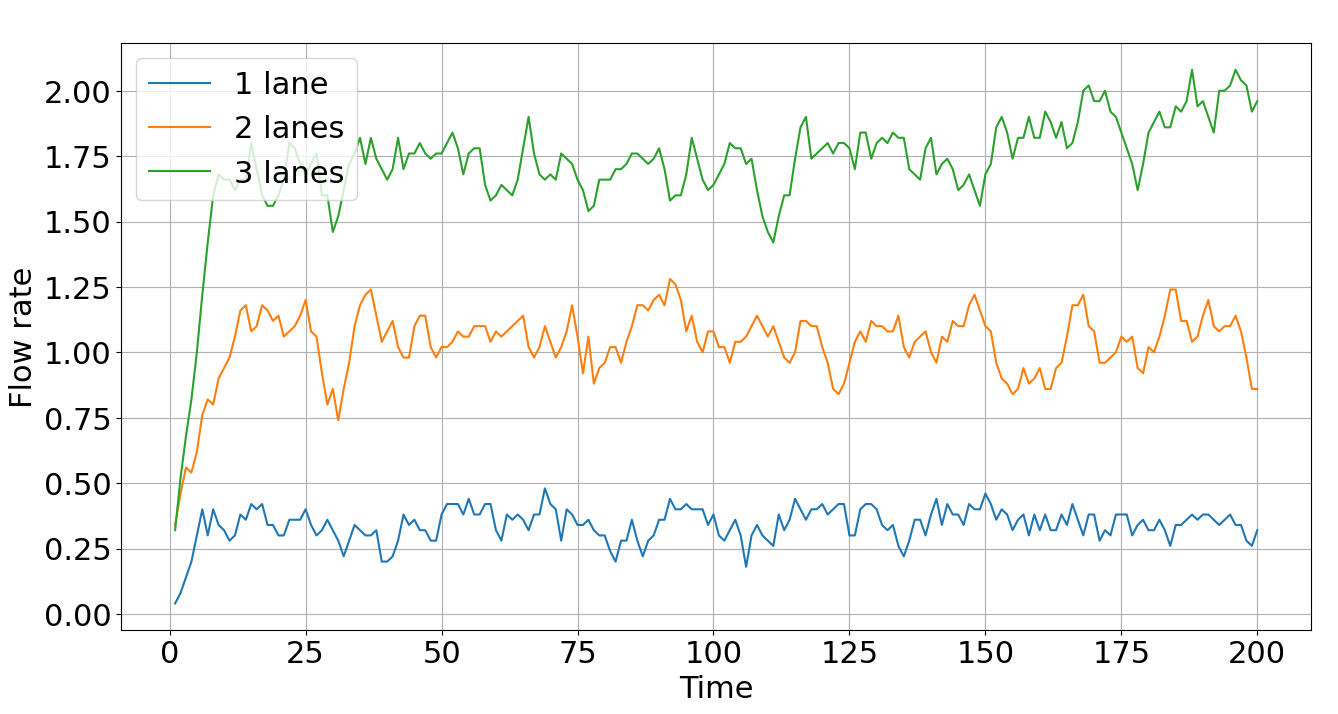
\includegraphics[scale=0.45]{fig1.png}
    \caption{Flow rate vs. time for different number of lanes, $n_{cars}=50$, L=100, $v_{road}=5$, p=0.2.}
    \label{fig1}
\end{figure}

\begin{center}
\def\arraystretch{1.5}
\begin{tabular}{ |c|c|c| } 
 \hline
	Number of lanes & \makecell{Mean flow rate} & \makecell{Max flow - min flow}\\
 \hline
	 1 & 0.35 & 0.28 \\
	 2 & 1.04 & 0.40 \\
	 3 & 1.80 &  0.66 \\
 \hline
\end{tabular}\\
\end{center}
Table 1: Mean flow rate and difference between maximum and minimum flow, calculated for the last 100 time steps for the simulation shown in figure \ref{fig1}.\\

Precision is investigated by doing multiple simulations like the one above. In figure \ref{semq} the standard error of the mean flow rate is shown as a function of the number of simulations. The error arises from the randomness in the assignment of max velocities and from the braking probability p. The error seems to be in the order of $10^{-2}$ for two lanes and 10 iterations, somewhat higher for three and lower for one. All of the errors decreases towards 0 as expected, approximately $\propto \frac{1}{\sqrt{n}}$. From now on we will use the mean of 10 iterations (and the mean of last 100 time steps for every iteration) for any measurement of an observable. 

\begin{figure}[H]
	 \centering
        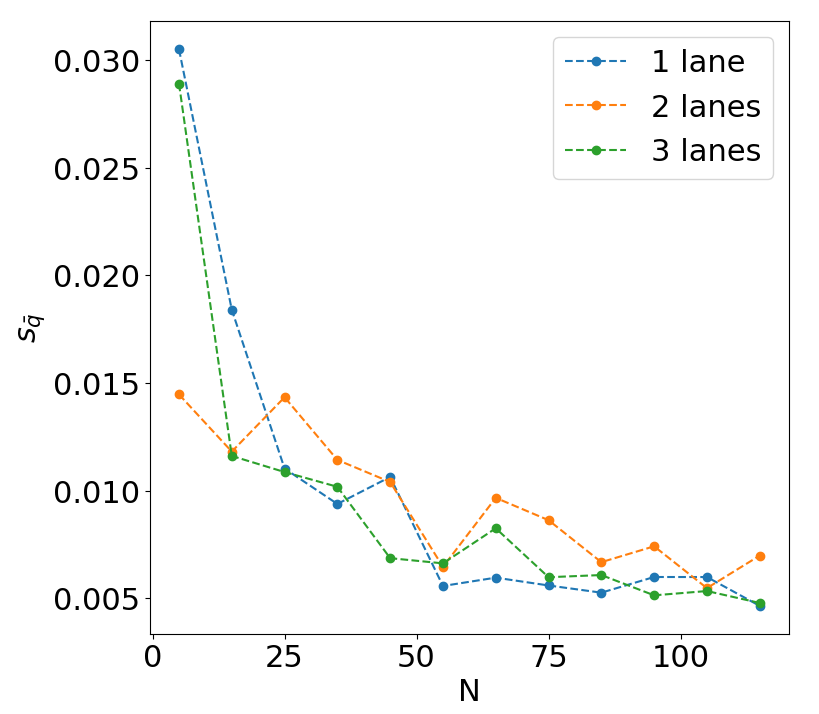
\includegraphics[scale=0.4]{fig6.png}
         \caption{Standard error of the mean flow rate $s_{\bar{q}}$ as a function of number of simulations N in a log-log plot. L=100, $n_{cars}=50$, p=0.2, $v_{road}=5$. A line $kN^{-0.5}$, (k is a suitable constant), is fitted to show the rate of decline.}
    \label{semq}
\end{figure}

\subsection{Fundamental Diagram}
The fundamental diagram of flow rate plotted against density of cars is an essential tool in traffic flow analysis. Here the goal is to fit a suitable model to describe this diagram. One of the oldest used models is the Greenshields model, which states that the flow rate depends on density as a second degree polynomial.\footnote{Pereira, Boyraz Baykas, Kulcsár et al., \textit{Parameter and density estimation from real-world traffic data: A kinetic compartmental approach}, \url{https://research.chalmers.se/publication/527726/file/527726_Fulltext.pdf}} In figure \ref{fig3} we have generated the fundamental diagram by simulating the system for different number of cars (where density $\rho = \frac{n_{cars}}{L}$) and calculated the flow rate. The fitted second degree polynomials are shown in table 2, and we see that it is not a good fit at all, which the low $R^2$-values also are indicators of.\\

\begin{figure}[H]
	\centering
        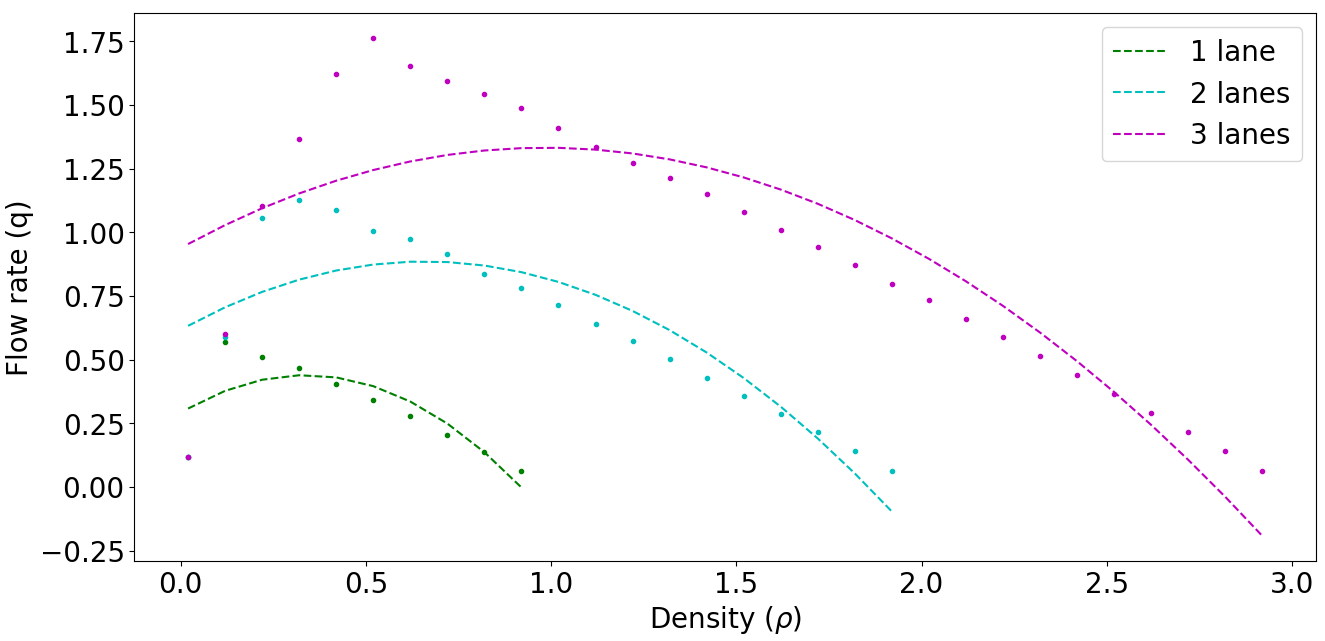
\includegraphics[scale=0.45]{fig3.png}
    \caption{Flow rate vs. density for different number of lanes and fitted second degree polynomials, L=100, $v_{road}=5$, p=0.2.}
    \label{fig3}
\end{figure}

\begin{center}
\def\arraystretch{1.5}
\begin{tabular}{ |c|c|c| } 
 \hline
	\makecell{Number of\\ lanes} & Regression curve & $R^2$ \\
 \hline
	 1 & $q= -1.30\rho^2+0.88\rho+0.29$  & 0.66016  \\
	 2 & $q= -0.62\rho^2+0.82\rho+0.62$ & 0.71849 \\
	 3 &$ q= -0.51\rho^2+0.81\rho+0.94 $& 0.73947 \\
 \hline
\end{tabular}\\
\end{center}
Table 2: Second degree polynomials fitted to fundamental diagram in figure \ref{fig3}, and corresponding $R^2$-values.\\

Another commonly used model is the triangular diagram, which models the fundamental diagram with two linear functions. In figure \ref{fig2} we have, for different number of lanes, fitted a line ($q = \alpha_1+\beta_1\rho$) for the points before the maximum recorded flow rate, and one line for the remaining part ($q = \alpha_2+\beta_2\rho$). The obtained parameter estimates (with 95\% confidence intervals) are shown in table 3, together with the $R^2$-values (calculated for the entire triangular curve, all points). These are very close to 1, which confirms that the fit is very good.\\

The flow rate approaches 0 for $\rho=i$ for a road with i lanes, which is to be expected as that means the road is completely full. It is also expected that q=0 when $\rho=0$, a hypotheses that cannot be rejected according to the confidence intervals for $\alpha_1$, all encompass 0. Furthermore, we see that the maximum flow rate more than doubles when going from 1 lane to 2, and it more than triples when going from 1 to 3. The critical density (where the flow rate starts to decrease) also increases with more lanes as can be seen in table 3. Another interesting fact is that the regression lines seem to be almost parallel for different number of lanes. Studying the confidence intervals for $\beta_1$ all intervals overlap, therefore the hypotheses that $\beta_1$ is constant for different number of lanes cannot be rejected. The same goes for the slope $\beta_2$.
\begin{figure}[H]
	\centering
        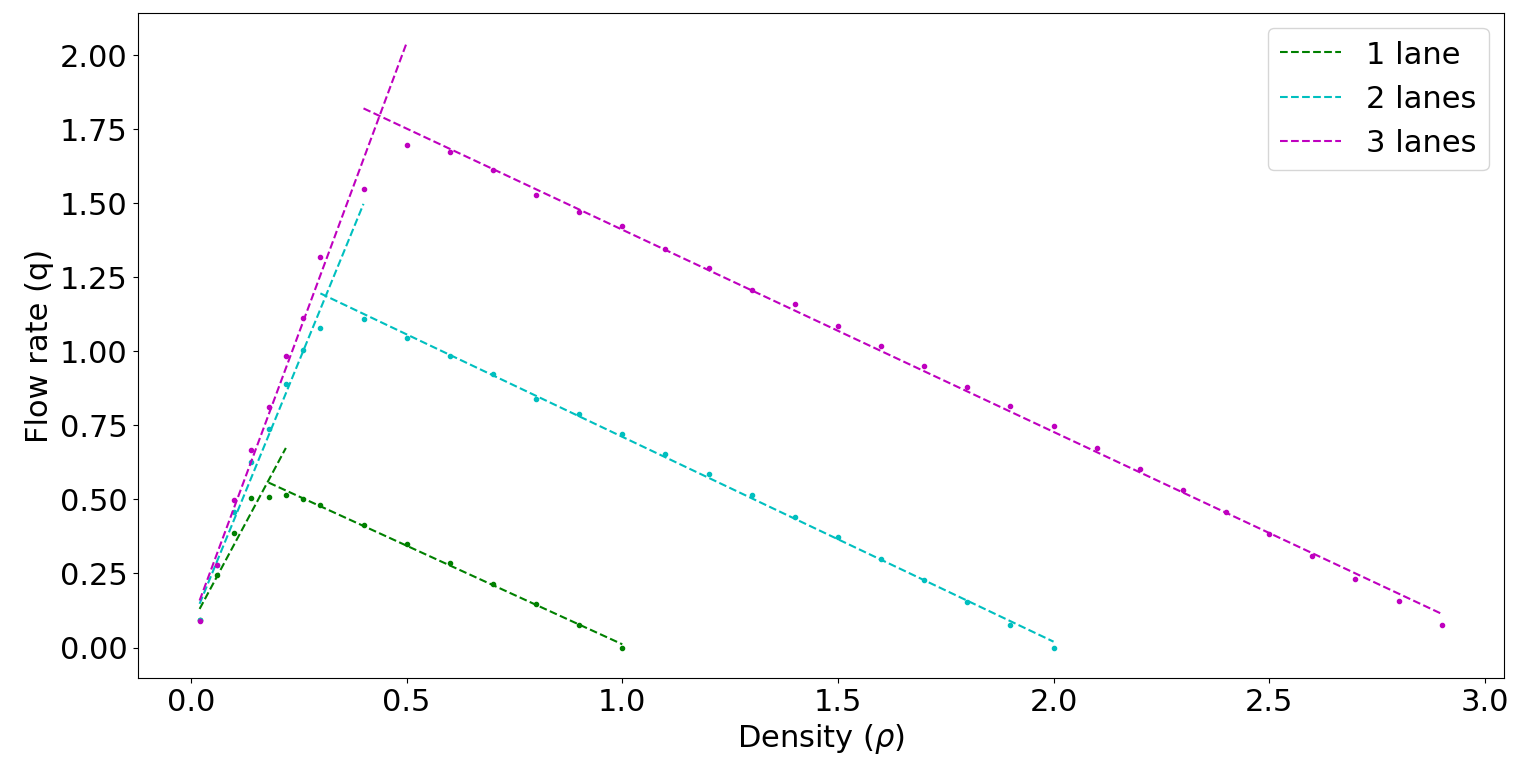
\includegraphics[scale=0.4]{fig22.png}
    \caption{Flow rate vs. density for different number of lanes, L=100, $v_{road}=5$, p=0.2.}
    \label{fig2}
\end{figure}

\begin{center}
\def\arraystretch{2.7}
\begin{tabular}{ |c|c|c|c|c|c| } 
 \hline
	\makecell{Number of \\lanes} & \makecell{Critical\\ density} &\makecell{Max flow rate \\ (predicted)} & \makecell{Regression curve \\$q=\alpha_1+\beta_1\rho$ \\(increase)} & \makecell{Regression curve \\ $q=\alpha_2+\beta_2\rho$  \\(decrease)} & $R^2$ \\
 \hline
	 1 & 0.178 & 0.558 &\makecell{$\alpha_1 = 0.076 \pm 0.153$ \\ $\beta_1 = 2.72 \pm 1.33$} & \makecell{$\alpha_2 = 0.676 \pm 0.020$ \\ $\beta_2 = -0.665 \pm 0.031$} & 0.97962  \\
	 2 & 0.313 & 1.19 & \makecell{$\alpha_1 = 0.077 \pm 0.078$ \\ $\beta_1 = 3.55 \pm 0.43$} & 
	 \makecell{$\alpha_2 = 1.40 \pm 0.02$ \\ $\beta_2 = -0.691 \pm 0.013$}  & 0.99508 \\
	 3 & 0.437 & 1.79 & \makecell{$\alpha_1 = 0.080 \pm 0.090$ \\ $\beta_1 = 3.92 \pm 0.41$} & 
	 \makecell{$\alpha_2 = 2.09 \pm 0.02$ \\ $\beta_2 = -0.682 \pm 0.013$} & 0.99576 \\
 \hline
\end{tabular}\\
\end{center}
Table 3: Critical density, predicted max flow rate and regression fits with 95\% confidence intervals, for the triangular model of fundamental diagram in figure \ref{fig2}.


\subsection{Proportion and velocity of cars in different lanes}

Simulating a 2-lane road for different densities, figure \ref{fig45} shows that for low densities most cars are in the inner lane (seems reasonable - no need for overtaking on an empty road). However, the share of cars in the second lane increases rapidly and for densities 0.5 and above there are roughly the same number of cars in both lanes, and the second lane even shows a tendency to be a bit more crowded. Furthermore, for low densities the mean velocity is higher in the second lane, but for densities above 0.5 the mean velocity is the same or lower compared to the first. This indicates that the passing lane is not faster in a traffic jam. 
\begin{figure}[H]
	 \centering
    \begin{minipage}{.5\textwidth}
        \centering
        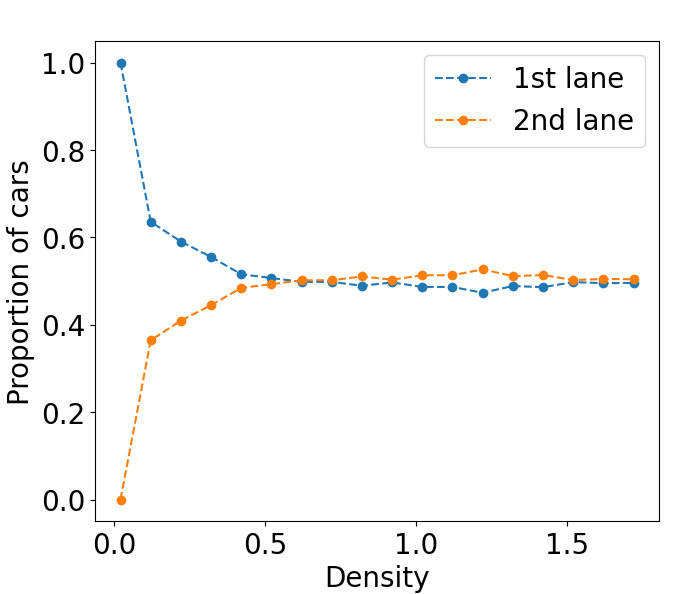
\includegraphics[scale=0.37]{fig5.png}
        \captionof*{figure}{Proportion of cars in lane vs. density}
    \end{minipage}%
    \begin{minipage}{.5\textwidth}
        \centering
        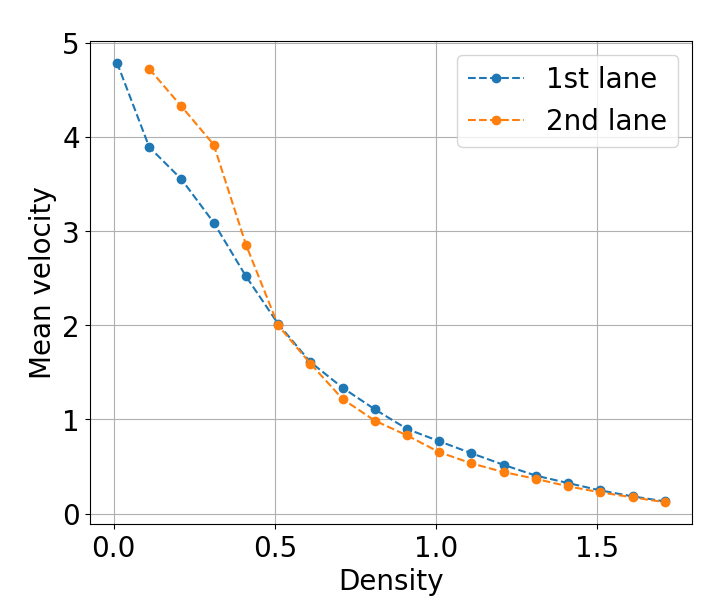
\includegraphics[scale=0.37]{fig4.png}
        \captionof*{figure}{Mean velocity in respective lane.}
    \end{minipage}
    \caption{Proportion and mean velocity of cars in 1st (inner) and 2nd (outer) lane for a 2-lane highway with L=100, $v_{road}=5$, p=0.2.}
    \label{fig45}
\end{figure}

For three lanes the behavior is similar. With few cars only the first lane is filled and as the road becomes more crowded the second and third lane become more populated (the third more slowly though). For high densities there seems to be a uniform distribution of cars among the three lanes, and while the mean velocity is higher in the second and third lane for low densities, they seem to be the same when the road is crowded.
\begin{figure}[H]
	 \centering
    \begin{minipage}{.5\textwidth}
        \centering
        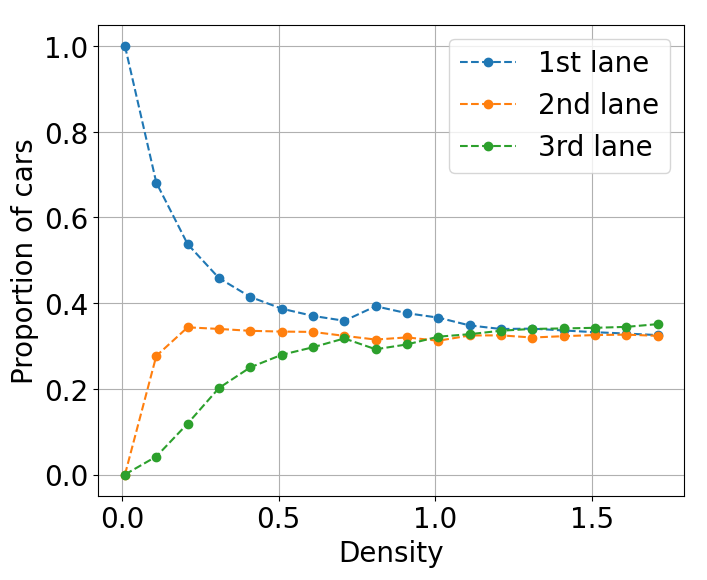
\includegraphics[scale=0.37]{fig8.png}
        \captionof*{figure}{Proportion of cars in lane vs. density}
    \end{minipage}%
    \begin{minipage}{.5\textwidth}
        \centering
        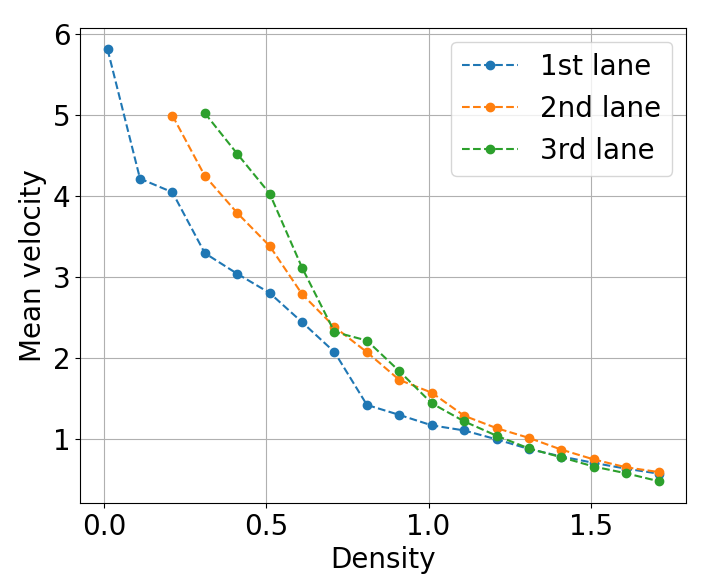
\includegraphics[scale=0.37]{fig9.png}
        \captionof*{figure}{Mean velocity in respective lane.}
    \end{minipage}
    \caption{Proportion and mean velocity of cars in 1st (inner), 2nd (middle) and 3rd (outer) lane for a 3-lane highway with L=100, $v_{road}=5$, p=0.2.}
    \label{41a}
\end{figure}

Now let us analyze the error in measurements of proportion and mean velocity. In figure \ref{sempv} below we see the SEM for the proportion of cars in the inner lane and the mean velocity in respective lane for a 2-lane road. Similarly as before the errors decrease as $N^{-0.5}$. For the proportion the SEM is in the order of 0.007 while for the mean velocity the error is around 0.05 for 10 simulations, which was used for each point in the diagrams above. 
\begin{figure}[H]
	 \centering
    \begin{minipage}{.5\textwidth}
        \centering
        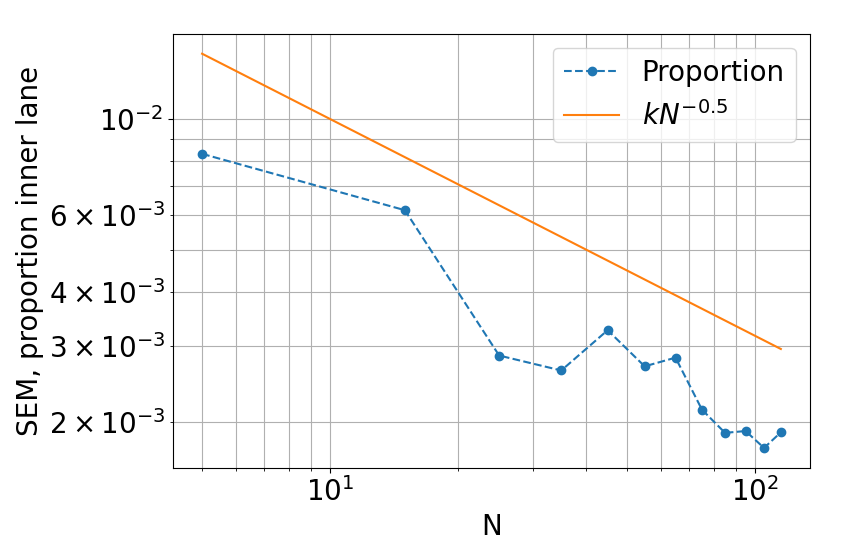
\includegraphics[scale=0.36]{fig11.png}
        \captionof*{figure}{Proportion of cars in inner lane}
    \end{minipage}%
    \begin{minipage}{.5\textwidth}
        \centering
        \includegraphics[scale=0.36]{fig12.png}
        \captionof*{figure}{Mean velocity}
    \end{minipage}
    \caption{SEM for proportion of cars in inner lane and mean velocity in respective lane for a 2-lane road, as a function of number of simulations N. L=100, $v_{road}=5$, p=0.2, $n_{cars}=50$.}
    \label{sempv}
\end{figure}


\subsection{Effect of velocity distribution on flow rate}

In figure \ref{fig10} below we see the flow rate as a function of the standard deviation used when generating the max velocities of the cars. The flow rate decreases the more spread out the velocities are (i.e. some want to drive really fast, some really slow). However, the flow rate decreases more with a single lane which corresponds with intuition - if there are several lanes one slow driver will not affect the entire traffic flow as much. 
\begin{figure}[H]
	\centering
        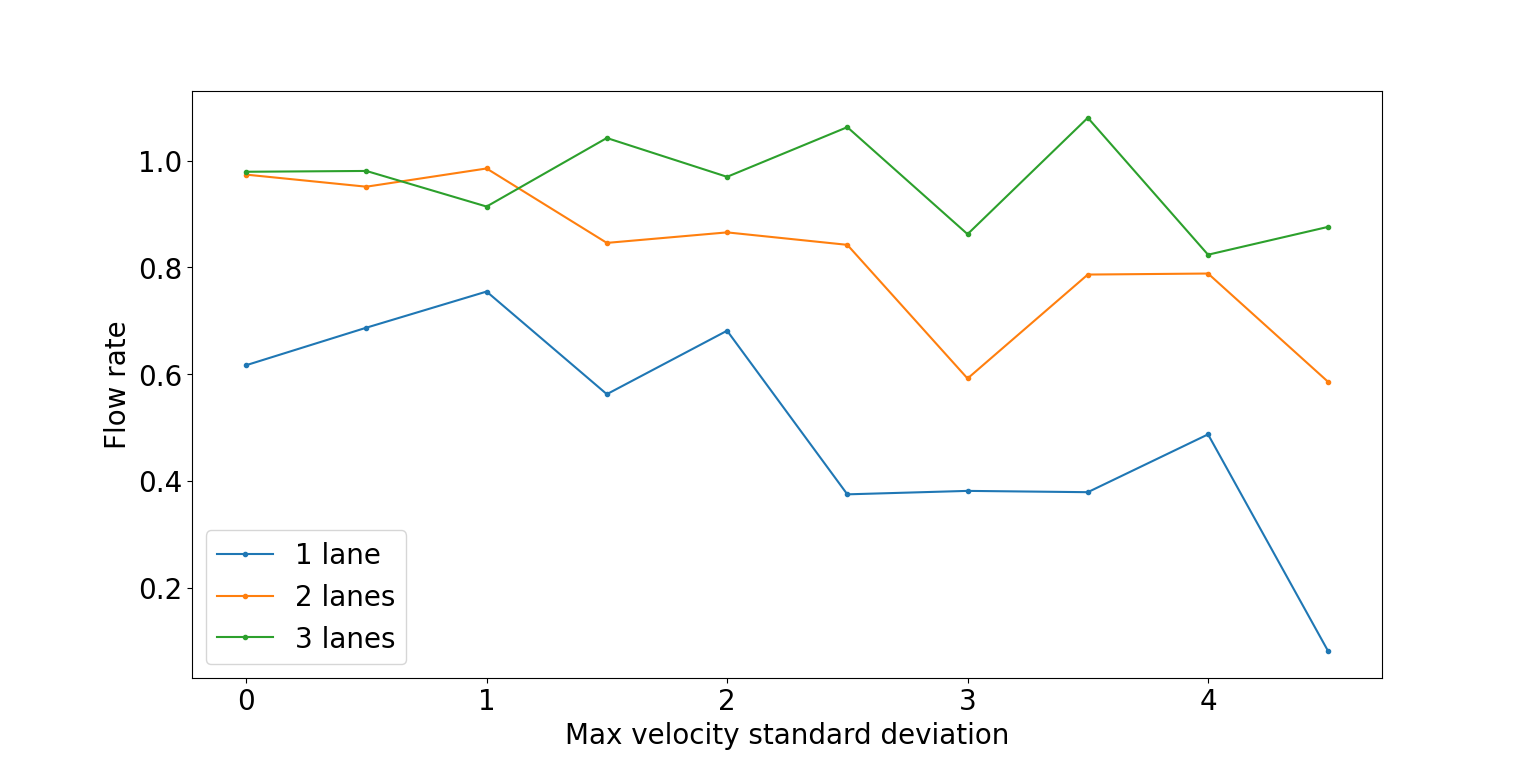
\includegraphics[scale=0.45]{fig10.png}
    \caption{Flow rate as a function of the maximum velocity standard deviation for a system with L=100, $n_{cars}=10$, $v_{road}=10$, p=0.2 and different number of lanes.}
    \label{fig10}
\end{figure}

\subsection{Discretization issues}
Using a cellular automaton model can yield some discretization issues. Here the road length is an important parameter, and in figure \ref{figrl} the fundamental diagram is plotted using different road lengths. The results seem to become quite independent of the road length somewhere around L=50. Therefore L=100, used in all simulations above, will yield rather small discretization errors. Of course an even longer road length would be optimal to use, but that would require more computing power.


\begin{figure}[H]
	 \centering
    \begin{minipage}{.5\textwidth}
        \centering
        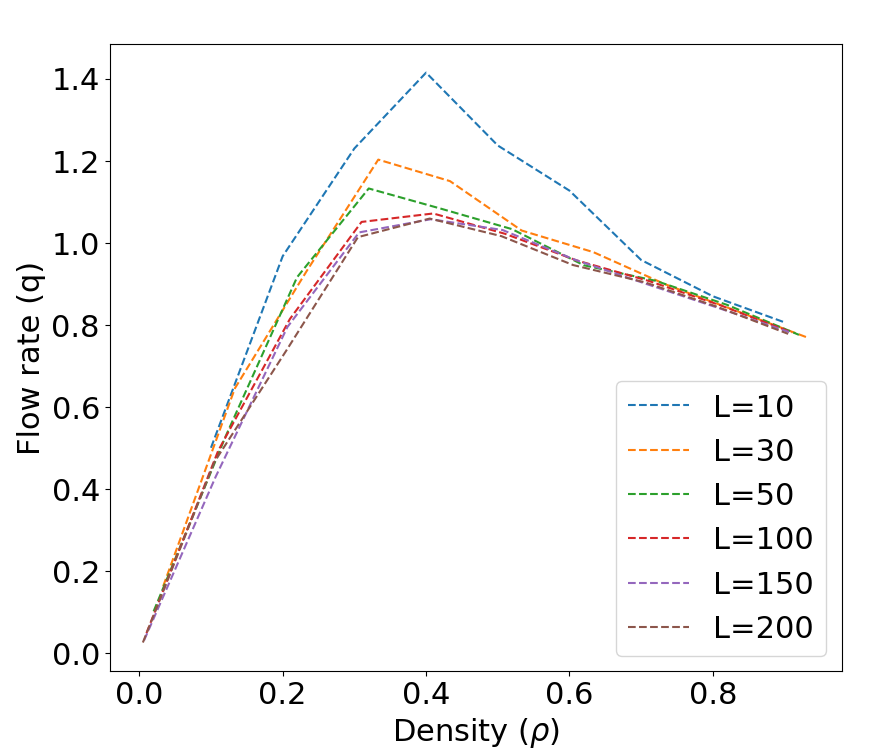
\includegraphics[scale=0.34]{figrl1.png}
        \captionof*{figure}{2 lanes}
    \end{minipage}%
    \begin{minipage}{.5\textwidth}
        \centering
        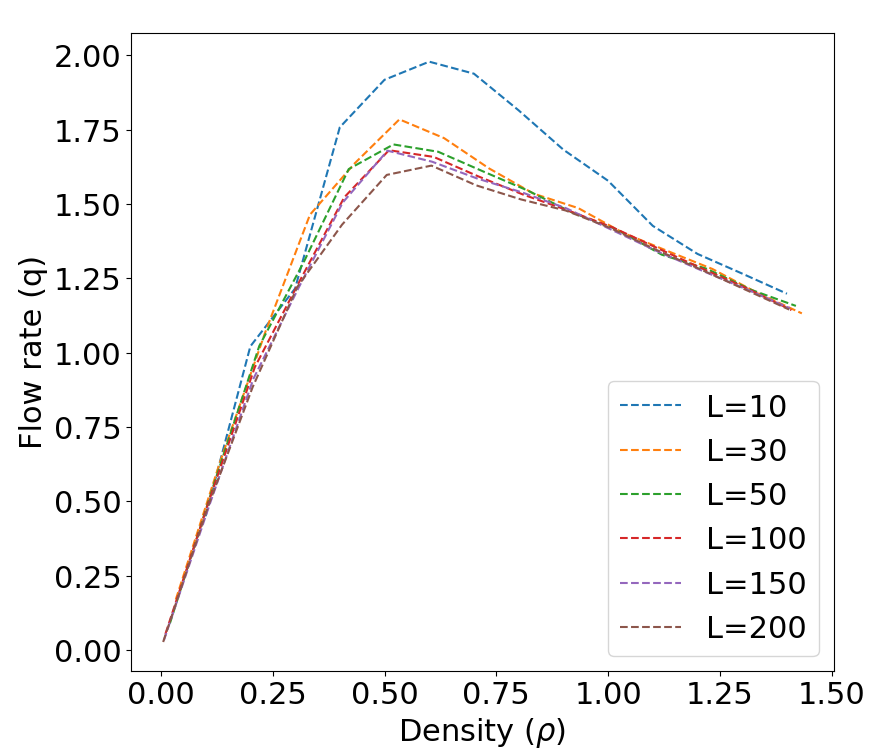
\includegraphics[scale=0.34]{figrl2.png}
        \captionof*{figure}{3 lanes}
    \end{minipage}
    \caption{Fundamental diagram with different road lengths L for two and three lane systems. $v_{road}=5$, p=0.2.}
    \label{figrl}
\end{figure}


\section{Accuracy \& precision}
The statistical precision has been examined using standard error for the observables and confidence intervals regression parameters. The rather high $R^2$ values for the triangular fundamental diagram model show that it provides a good description of the data. The plots of standard error for the flow rate, proportion and mean velocity seem to be in the order of $10^{-2}$, 0.007 and 0.05 respectively for 10 simulations and a 2-lane system, and it decreases with more simulations. More simulations would have yielded more precise answers, but required too much computing power. Furthermore, using for example a fixed velocity distribution instead of a random one would lead to more precise results, however the experiments would be less accurate in the description of reality. The accuracy of the simulation has been briefly discussed in section 2, but checking the results against real traffic data would be necessary to validate how well the model describes reality. 


\section{Appendix}
\subsection*{Some simulation videos}
\url{https://1drv.ms/u/s!As6qZQ3lM1amla5u7cvLu_ObiUkmHA?e=csYeen}

%\lstinputlisting[language=python]{codelistings.py}

 

\end{document}